\documentclass[convert={outext=.svg,command=\unexpanded{pdf2svg \infile\space\outfile}},multi=false]{standalone}

\usepackage{auto-pst-pdf}
\usepackage{pst-optic}

\usepackage{arev}
\usepackage[T1]{fontenc}
\usepackage{soul}

\begin{document}

%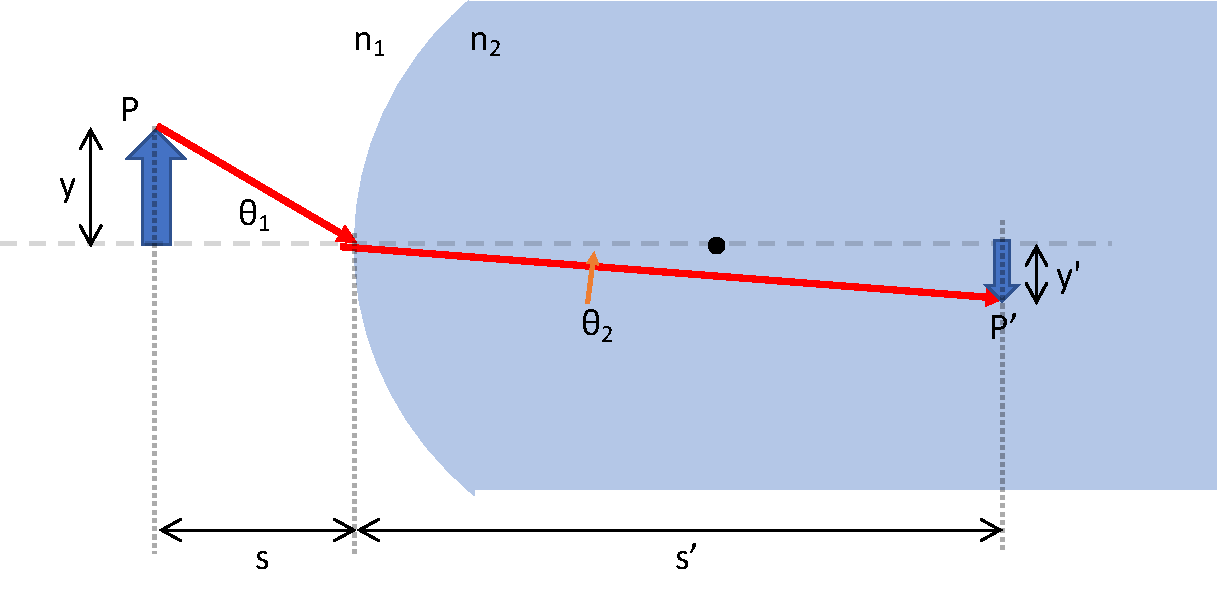
\includegraphics[scale=0.7]{ch16-sphsurfacemag}

\begin{pspicture}[showgrid=false](-10,-2.2)(7,4) 
\rput(0,0){%
\newpsstyle{opticalAxis}{linewidth=0.5pt,linecolor=gray,linestyle=dashed}
\lens[
lensType=CVG,
lensGlass,
lensWidth=0.5,
rayColor=red, 
focus=2.5,
AB=2,
OA=-7,
spotO=270,
spotAi=90,
spotBi=270,
spotFi=100,
nameFi=F',
]}
\psdot*(0,0)
\psline{|<->|,gray}(0,-2)(-7,-2)
\uput[d](-3.5,-2){$s$}
\psline{|<->|,gray}(0,-2)(3.95,-2)
\uput[d](1.75,-2){$s'$}

\psline{|<->|,gray}(-7.5,0)(-7.5,2)
\uput[l](-7.5,1){$y$}
\psline{|<->|,gray}(4.2,0)(4.2,-1.1)
\uput[r](4.2,-0.5){$y'$}

\uput[](-1.75,0.25){$\theta$}
\uput[](1.75,-0.25){$\theta$}
%\ncline{<->}{lens}{object}
%\uput[d](-3,0){F}
\end{pspicture}

\end{document}